\documentclass[notitlepage]{math}
\usepackage{lipsum}
\usetikzlibrary{patterns,positioning, decorations, decorations.pathreplacing}
\title{Vector Spaces Chap. 11} %Titre du fichie
\author{FireGhost} %Auteur du fichier

\begin{document}
\titre{Chapter 11: Vector Spaces} %Titre du fichier .pdf
\UE{Vector Spaces} %Nom de la UE

\fairetitre
\fairemarges
% subsubsubsection
\setcounter{secnumdepth}{4}
\titleformat{\paragraph}
{\normalfont\normalsize\bfseries}{\theparagraph}{1em}{}
\titlespacing*{\paragraph}
{0pt}{3.25ex plus 1ex minus .2ex}{1.5ex plus .2ex}

\newcommand{\minus}{\scalebox{0.75}[1.0]{$-$}} % Minus sign

During this chapter, $\mathbb{K}$ will be either $\mathbb{R}$ or $\mathbb{C}$.
\section{General approach}
\subsection{Structure of a Vector Space}
Let $E$ be a set, we define two operations:\\
\newline
\begin{minipage}{0.5\linewidth}
    \begin{itemize}
    \item An internal operation: \\
    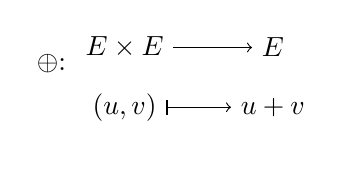
\begin{tikzpicture}[node distance=1mm]
        \node (center) at (0,0) {};
        \node (functionName) at (0, 1) {$\oplus$:};
        \node[above right = -0.3cm and 0cm of functionName] (domain) {$E \times E$};
        \node[right = 1cm of domain] (codomain) {$E$};
        \node[below = 2mm of domain] (element) {$(u , v)$};
        \node at (element-|codomain) (image) {$u+v$};
        \draw[->] (domain) -- (codomain);
        \draw[|->] (element) -- (image);
    \end{tikzpicture}
\end{itemize}
\end{minipage}
\begin{minipage}{0.5\linewidth}
    \begin{itemize}
    \item An external operation: \\
    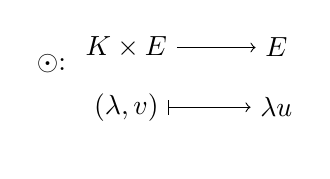
\begin{tikzpicture}[node distance=1mm]
        \node (center) at (0,0) {};
        \node (functionName) at (0, 1) {$\odot$:};
        \node[above right = -0.3cm and 0cm of functionName] (domain) {$\mathbb{K} \times E$};
        \node[right = 1cm of domain] (codomain) {$E$};
        \node[below = 2mm of domain] (element) {$(\lambda , v)$};
        \node at (element-|codomain) (image) {$\lambda u$};
        \draw[->] (domain) -- (codomain);
        \draw[|->] (element) -- (image);
    \end{tikzpicture}
\end{itemize}
\end{minipage}
\subsection{Defintion}
\noindent We say that $(E, \oplus, \odot)$ is a vector space if $\forall (u,v,w) \in E^3$ we have:
\begin{itemize}
    \item u + (v + w) = (u + v) + w {\color{green}($\oplus$ is associative)}
    \item u + v = v + u {\color{green}($\oplus$ is commutative)}
    \item $\exists 0_E \in E$ such that $u + 0_E = 0_E + u = u$ {\color{green}(Existence of a neutral element for $\oplus$)}
    \item $\exists \minus u \in E$, $u + (\minus u) = (\minus u) + u = 0_E$ {\color{green}(Existence of a symmetrical element for $\oplus$)}
\end{itemize}
And $\forall (u, v) \in E^2$ and $\forall (\alpha, \beta) \in \mathbb{K}^2$ we have:
\begin{itemize}
    \item $(\alpha + \beta) \cdot u = \alpha \cdot u + \beta \cdot u$ {\color{green}($\odot$ is distributive)}
    \item $\alpha (u + v) = \alpha \cdot u + \alpha \cdot v$ {\color{green}($\odot$ is distributive)}
    \item $(\alpha \beta) u = \alpha (\beta u)$ {\color{green}($\odot$ is associative)}
    \item $1_{\mathbb{K}} \cdot u = u$ {\color{green}(Where $1_{\mathbb{K}}$ is the neutral element of multiplication of element of $\mathbb{K}$)}
\end{itemize}
Let (E, $\oplus$, $\odot$) be a $\mathbb{K}$-Vector Space,\\
Any element from E is called a vector and any element from $\mathbb{K}$ is called a scalar.\\
$0_E$ is called the zero vector.\\
\subsubsection{Property}
$\forall u \in E$ and $\forall \alpha \in \mathbb{K}$ we have:
\begin{enumerate}
    \item $\alpha \cdot 0_E = 0_E$
    \item $0_{\color{red}\mathbb{K}} \cdot u = 0_{\color{red}E}$
    \item $\alpha \cdot u = 0_E \Leftrightarrow \alpha = 0_{\color{red}\mathbb{K}}$ or $u = 0_{\color{red}E}$
\end{enumerate}
\subsubsection{Example}
...
\subsection{Vector Subspaces (= linear subspaces)}
\subsubsection{Definition}
Let $E$ be a $\mathbb{K}$-Vector Space:\\
\begin{itemize}
    \item $F \subset E$ {\color{green}(F is a subset of E)}
    \item $F \neq \emptyset$ {\color{green}(F is non-empty, $0_E \in F$)}
    \item $\forall (u, v) \in F^2$, $\forall \alpha \in \mathbb{K}$, $(\alpha \cdot u + v) \in F$ {\color{green}(F is closed under linear combination)}
\end{itemize}
\subsubsection{Propositions}
\paragraph{Proposition 1}
Let $E$ be a $\mathbb{K}$-Vector Space:
\begin{align*}
    F \subset E \text{ is a Vector SubSpace of } E &\Longrightarrow 0_E \in F\\
    &\;\not\!\!\!\Longleftarrow  
\end{align*}
\paragraph{Example}
\noindent $E = \mathbb{R}^3$\\
$F_1 = \left\{\begin{pmatrix} x\\ y\\ z \end{pmatrix} \in \mathbb{R}^3, x + y + z = 1\right\}$ and $F'_1 = \left\{\begin{pmatrix} x\\ y\\ z \end{pmatrix} \in \mathbb{R}^3, x + y + z = 0\right\}$\\
$0_E \notin F_1 \Longrightarrow F_1$ is not a Vector SubSpace of $E$\\
$\forall (u, v) \in {F'}_1^2$, $\forall \alpha \in \mathbb{R}$, $u = \begin{pmatrix} x\\ y\\ z \end{pmatrix}$ and $v = \begin{pmatrix} x'\\ y'\\ z' \end{pmatrix}$\\
$\alpha u + v = \alpha(x, y, z) + (x', y', z') = 0_E \in F'_1$
$\Longrightarrow F'_1$ is a Vector SubSpace of $E$
{\color{blue}TODO A MINIPAGE FOR THE EXAMPLE AND ADD THE OTHER EXAMPLES}
\paragraph{Proposition 2}
Let $E$ be a Vector Space, $F$ and $G$ two Vector SubSpaces of $E$. Then:\\
\begin{enumerate}
    \item $F \cap G \subset E$,    $F \cap G$ is a Vector SubSpace of $E$
    \item {\color{blue}TO FINISH}
\end{enumerate} 
\end{document}